\begin{frame}
	\frametitle{Project Background}
	Nuclear fusion -- the energy of the future!
    \vspace{10pt}
	\begin{itemize}
	    \item Must produce and contain an extremely hot and dense plasma
	    \begin{itemize}
		    \item Magnetic Confinement Fusion (MCF): toroidal circulation
		    \item Inertial Confinement Fusion (ICF): spherical compression
		\end{itemize}
		\vspace{10pt}
		\item Modern designs require enriched Hydrogen fuel of two varieties:
	    \begin{itemize}
		    \item Deuterium ($^2$H) -- abundant in naturally-sourced water
		    \item Tritium ($^3$H) -- extremely rare, but can be produced \textit{in-reactor}
		\end{itemize}
	\end{itemize}
	\vspace{10pt}
	\centering{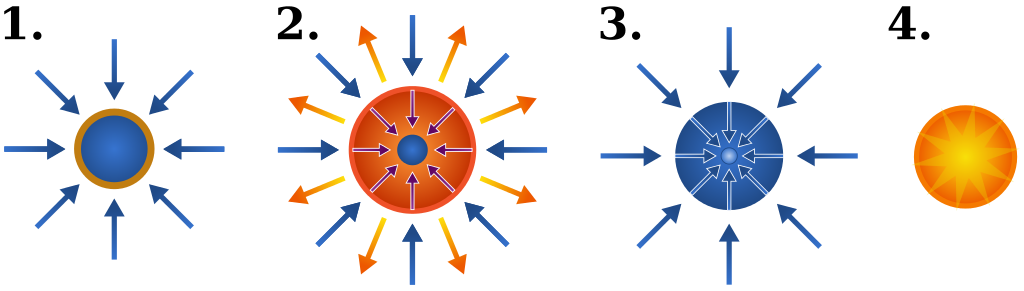
\includegraphics[height=3cm]{icf_diagram}}
\end{frame}

\begin{frame}
	\frametitle{Problem Description}
	\begin{itemize}
		\item % TODO
	\end{itemize}
\end{frame}

\begin{frame}
	\frametitle{Data Generation}
	\begin{itemize}
		\item % TODO
	\end{itemize}
\end{frame}

%\begin{frame}
%	\frametitle{Dimensionality Reduction}
%	\begin{itemize}
%		\item % TODO
%	\end{itemize}
%\end{frame}

\begin{frame}
	\frametitle{Methodology}
			Conventional regression task -- search for a cheap surrogate $\hat{f}(x)$ that
			minimizes dissimilarity with an expensive function $f(x)$:

			\begin{itemize}
				\item
					Regression performance (capability to approximate)
					\begin{itemize}
						\item Absolute: mean absolute error, $\sigma$ of error
						\item Relative: $R^2$, $R^2_\text{adj.}$
					\end{itemize}
				\item
					Computational complexity:
					wall training \& prediction time / sample.
			\end{itemize}

			2 approaches for surrogate training:
			\begin{enumerate}
				\item
					Decoupled -- trains models from previously sampled
					$\mathcal{T}=\{(x,f(x))\}$.
				\item
					Adaptive -- repeats sampling \& model training, increases
					sampling density in low-performance regions.
			\end{enumerate}
\end{frame}

